\section{The source and the site}
\label{sec:source}

William wrote a century after the flight and could have heard it from men who knew Eilmer
\autocite{white1961eilmer,thomson2004eilmer_odnb}.
Supplementary S1 gives his Latin and a standard translation.
He says Eilmer ``collected the breeze on the summit of a tower'' and that the violence
of the wind and the swirling of the air brought him down.
The traditional date is about 1000--1010.
\textcite{aitcheson2026date} argues it could be as late as the early 1040s.
Launch weather is sampled from a modern climatology, so the year does not matter.

Other early flight accounts are mostly legend \autocite{paz2013humanflight}.
The only one with a stated device is that of Abbas ibn Firnas of ninth-century Córdoba,
whom later Andalusian chronicles credit with a structure of feathers and silk and a bad
landing, also blamed on a missing tail \autocite{white1961eilmer,anderson2024bridge}.
\textcite{hallion2003takingflight} reads it as closer to a parachute descent.
Neither gives dimensions or construction.
With no historical basis for a specific design, the models sample wing area, mass, shape,
and drag over wide ranges (Supplementary \cref{tab:priors}).

\begin{figure}[htbp]
  \centering
  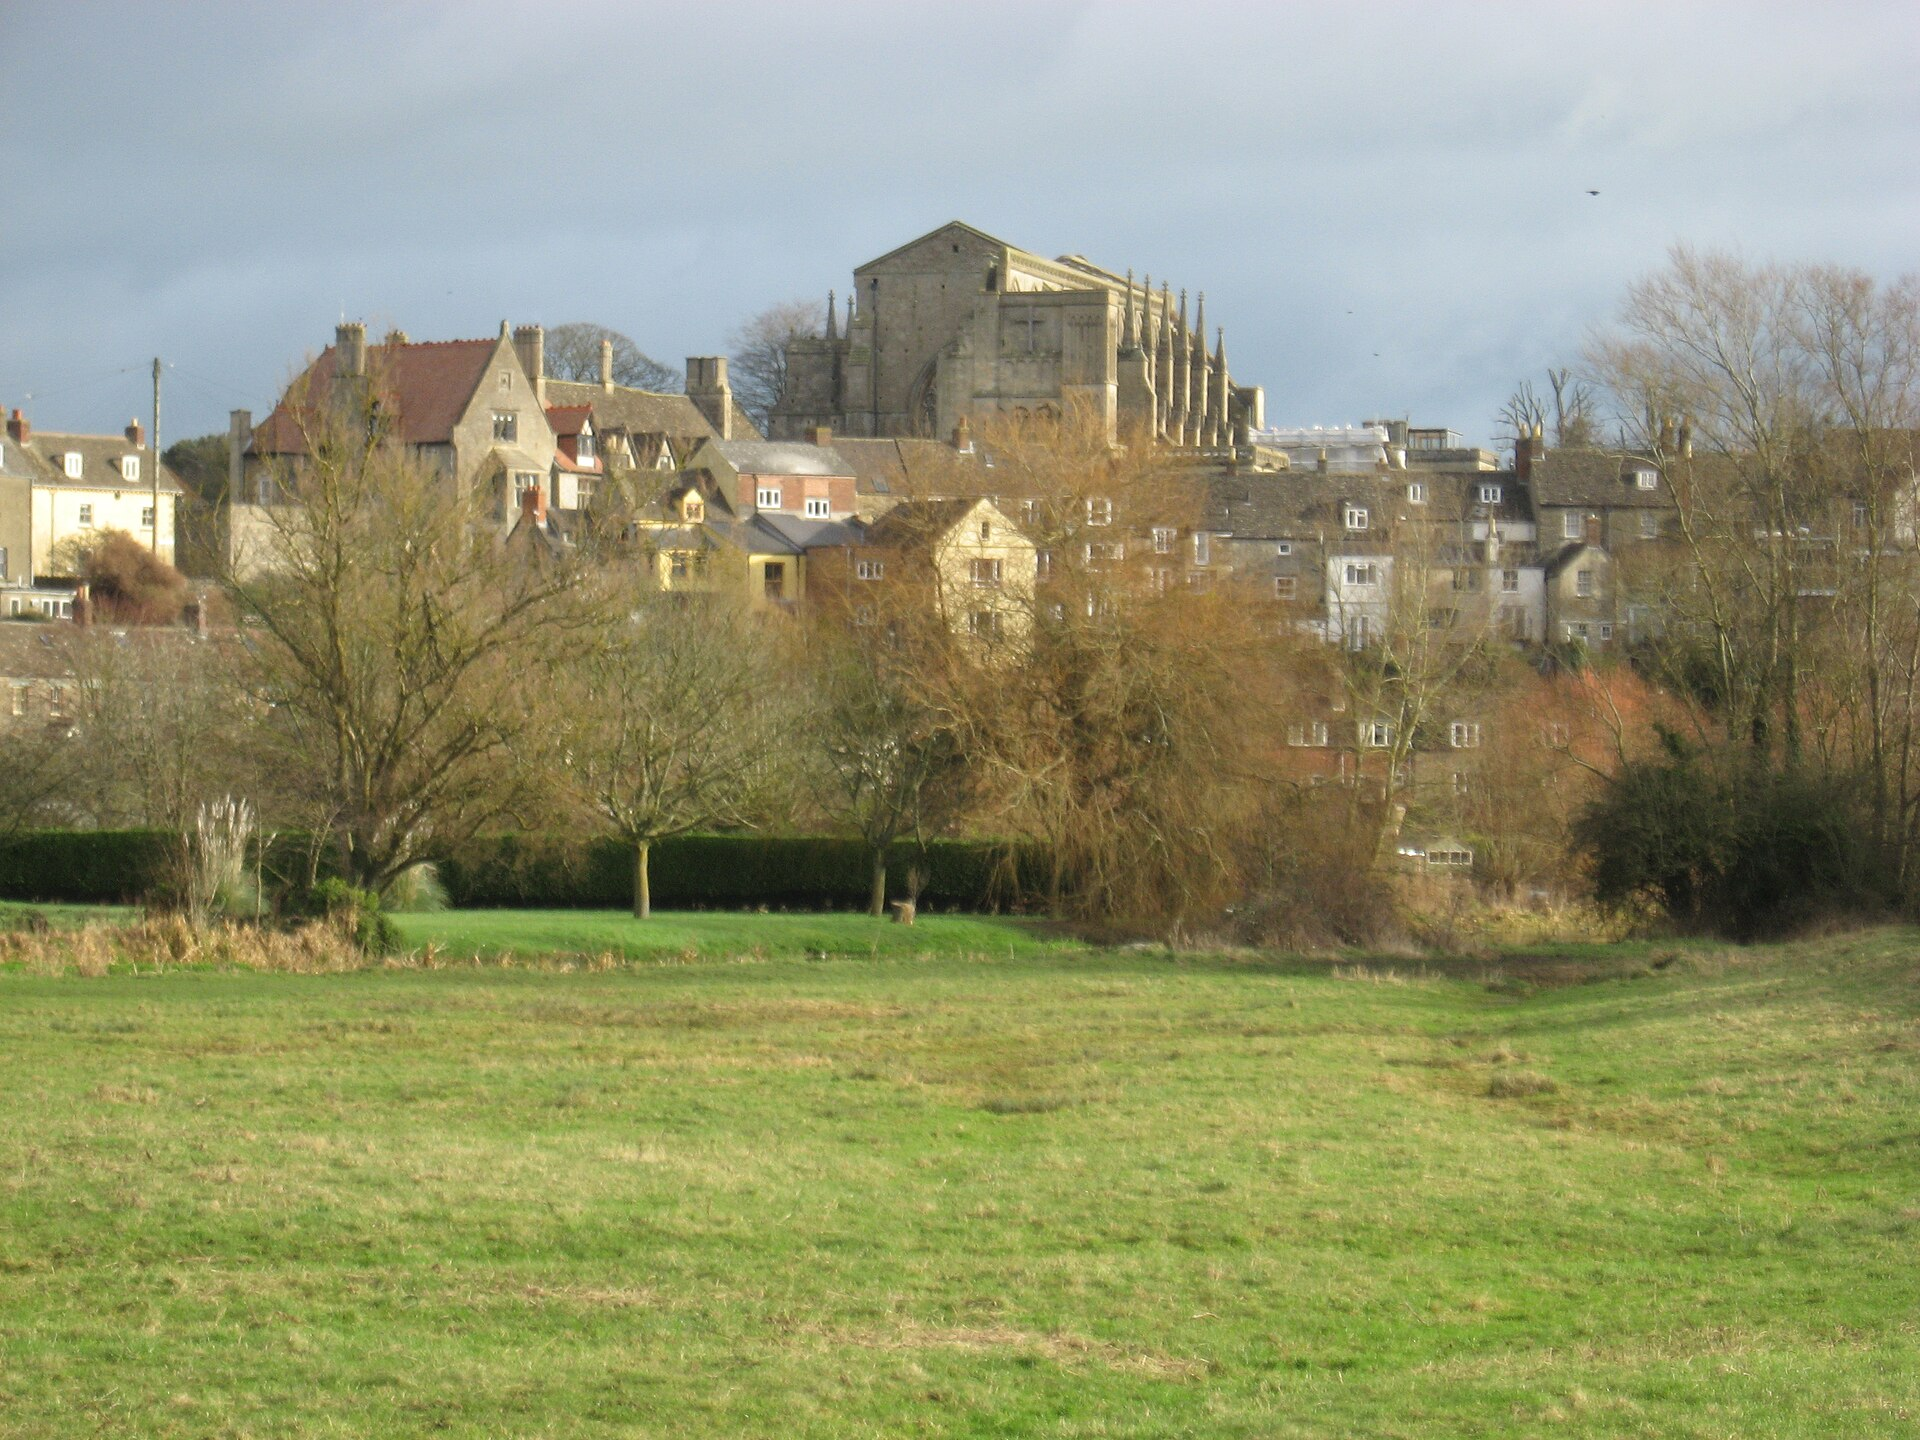
\includegraphics[width=0.8\linewidth]{fig_abbey_photo.jpg}
  \caption{\textbf{Malmesbury Abbey seen from the southwest.}
  The view looks northeast from the Avon water meadows, about \SI{300}{\meter} west-southwest
  of the abbey, up the slope the prevailing wind strikes.
  The present church is twelfth-century; Eilmer's Anglo-Saxon church and tower do not
  survive, so the launch point is taken as the abbey site and the tower height is sampled.
  Photograph: Dr Duncan Pepper (2012, Geograph and Wikimedia Commons), CC BY-SA 2.0.}
  \label{fig:photo}
\end{figure}

The abbey stands on a narrow spur between two arms of the Avon.
The sampled tower height, \SIrange{\nTowerLo}{\nTowerHi}{\meter}, brackets White's estimate of about
\SI{\nTower}{\meter} \autocite{white1961eilmer}.
\textcite{woosnam1986eilmer} puts the flight down the steep slope southwest of the abbey
towards the river, the side shown in \cref{fig:photo}.
